\chapter{Design}

\section{Overall System Design}

\subsection{Short description of the main parts of the system}

\subsection{System flowcharts showing an overview of the complete system}

\section{User Interface Designs}

\section{Hardware Specficiation}
A computer was donated to the shop last June. This computer is a Dell desktop computer, with 1080p monitor and accessories, running Windows 7 Home Edition. 8GBs of DDR3 RAM, an i5 Intel processor, and a AMD video card. Judy has said that she is perfectly happy to us this computer as a work PC, along with being able to work on it all day. Looking at a technical standpoint of the components, it is more than enough to satisfy whatever my program needs, as my program will take up very little processing power, and require very little storage space, for both the program data itself and the database.

The program will run on a reasonably modern Dell desktop computer, with 1080p monitor and accessories, running Windows 7 Home Edition. 8GBs of DDR3 RAM, an i5 Intel processor, and a AMD video card.This system uses a traditional mouse and keyboard as a input system. Choices will be made by using the mouse to click buttons, and data is inputted by typing on the keyboard. The screen resolution provides plenty of space for a large GUI, if such a size is required. The program will be stored on the computer's hard drive (500Gbs), which will provide plenty

\section{Program Structure}

\subsection{Top-down design structure charts}

\subsection{Algorithms in pseudo-code for each data transformation process}

\subsection{Object Diagrams}

\subsection{Class Definitions}

\section{Prototyping}

\section{Definition of Data Requirements}

\subsection{Identification of all data input items}

\subsection{Identification of all data output items}

\subsection{Explanation of how data output items are generated}

\subsection{Data Dictionary}

\subsection{Identification of appropriate storage media}

\section{Database Design}

\subsection{Normalisation}

\subsubsection{ER Diagrams}
\begin{figure}[H]
    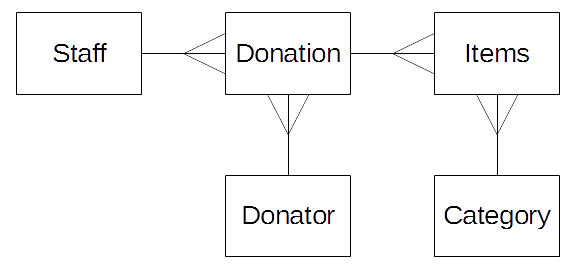
\includegraphics[width=\textwidth]{./Design/Images/ERDiagram.png}
\end{figure}

\subsubsection{Entity Descriptions}
Staff(\underline{StaffID},StaffFirstName,StaffLastName)
Category(\underline{ItemCategory},ItemCategoryDescription)
Item(\underline{ItemCode},ItemDescription,ItemPrice,\textit{ItemCategory},ItemQualityCheck,ItemStatus)
Donator(\underline{DonatorID},DonatorFirstName,DonatorLastName,DonatorAddress1,DonatorAddress2,DonatorCity,DonatorCounty,DonatorPostCode,DonatorContact)
Donation(\underline{DonationCode},\textit{ItemCode},\textit{DonatorID},\textit{StaffID},Date)

\subsubsection{1NF to 3NF}
\begin{center}
    \begin{tabular}{|p{4cm}|p{4cm}|}
	\hline
	\multicolumn{2}{|c|}{UNF} \\
	\hline
	\textbf{DonationCode} & \textbf{DonatorLastName} \\ \hline
	\textbf{Date} & \textbf{DonatorAddress1} \\ \hline
	\textbf{ItemDescription} & \textbf{DonatorAddress2} \\ \hline
	\textbf{ItemPrice} & \textbf{DonatorCity} \\ \hline
	\textbf{ItemCategory} & \textbf{DonatorCounty} \\ \hline
	\textbf{ItemCategoryDescription} & \textbf{DonatorPostCode} \\ \hline
	\textbf{ItemQualityCheck} & \textbf{DonatorDontact} \\ \hline
	\textbf{ItemCode} & \textbf{StaffFirstName} \\ \hline
	\textbf{ItemStatus} & \textbf{StaffLastName} \\ \hline
	\textbf{DonatorID} & \textbf{StaffID} \\ \hline
	\textbf{DonatorFirstName} \\ \hline
    \end{tabular}
\end{center}
	

\subsection{SQL}

\section{Security and Integrity of the System and Data}

\subsection{Security and Integrity of Data}

\subsection{System Security}

\section{Validation}

\section{Testing}

\begin{landscape}
\subsection{Outline Plan}

\begin{center}
    \begin{tabular}{|p{2cm}|p{5cm}|p{5cm}|p{4cm}|}
        \hline
        \textbf{Test Series} & \textbf{Purpose of Test Series} & \textbf{Testing Strategy} & \textbf{Strategy Rationale}\\ \hline
        Example & Example & Example & Example \\ \hline
    \end{tabular}
\end{center}

\subsection{Detailed Plan}

\begin{center}
    \begin{longtable}{|p{1.5cm}|p{2.5cm}|p{2.5cm}|p{2cm}|p{2cm}|p{2cm}|p{2cm}|p{2cm}|}
        \hline
        \textbf{Test Series} & \textbf{Purpose of Test} & \textbf{Test Description} & \textbf{Test Data} & \textbf{Test Data Type (Normal/ Erroneous/ Boundary)} & \textbf{Expected Result} & \textbf{Actual Result} & \textbf{Evidence}\\ \hline
        Example & Example & Example & Example & Example & Example & Example & Example \\ \hline
    \end{longtable}
\end{center}
\end{landscape}
